%% Beginning of file 'sample63.tex'
%%
%% Modified 2019 June
%%
%% This is a sample manuscript marked up using the
%% AASTeX v6.3 LaTeX 2e macros.
%%
%% AASTeX is now based on Alexey Vikhlinin's emulateapj.cls 
%% (Copyright 2000-2015).  See the classfile for details.

%% AASTeX requires revtex4-1.cls (http://publish.aps.org/revtex4/) and
%% other external packages (latexsym, graphicx, amssymb, longtable, and epsf).
%% All of these external packages should already be present in the modern TeX 
%% distributions.  If not they can also be obtained at www.ctan.org.

%% The first piece of markup in an AASTeX v6.x document is the \documentclass
%% command. LaTeX will ignore any data that comes before this command. The 
%% documentclass can take an optional argument to modify the output style.
%% The command below calls the preprint style which will produce a tightly 
%% typeset, one-column, single-spaced document.  It is the default and thus
%% does not need to be explicitly stated.
%%
%%
%% using aastex version 6.3.1
\documentclass{aastex631}

%% For wrapping figures in text
\usepackage{wrapfig}

%% The default is a single spaced, 10 point font, single spaced article.
%% There are 5 other style options available via an optional argument. They
%% can be invoked like this:
%%
%% \documentclass[arguments]{aastex63}
%% 
%% where the layout options are:
%%
%%  twocolumn   : two text columns, 10 point font, single spaced article.
%%                This is the most compact and represent the final published
%%                derived PDF copy of the accepted manuscript from the publisher
%%  manuscript  : one text column, 12 point font, double spaced article.
%%  preprint    : one text column, 12 point font, single spaced article.  
%%  preprint2   : two text columns, 12 point font, single spaced article.
%%  modern      : a stylish, single text column, 12 point font, article with
%% 		  wider left and right margins. This uses the Daniel
%% 		  Foreman-Mackey and David Hogg design.
%%  RNAAS       : Preferred style for Research Notes which are by design 
%%                lacking an abstract and brief. DO NOT use \begin{abstract}
%%                and \end{abstract} with this style.
%%
%% Note that you can submit to the AAS Journals in any of these 6 styles.
%%
%% There are other optional arguments one can invoke to allow other stylistic
%% actions. The available options are:
%%
%%   astrosymb    : Loads Astrosymb font and define \astrocommands. 
%%   tighten      : Makes baselineskip slightly smaller, only works with 
%%                  the twocolumn substyle.
%%   times        : uses times font instead of the default
%%   linenumbers  : turn on lineno package.
%%   trackchanges : required to see the revision mark up and print its output
%%   longauthor   : Do not use the more compressed footnote style (default) for 
%%                  the author/collaboration/affiliations. Instead print all
%%                  affiliation information after each name. Creates a much 
%%                  longer author list but may be desirable for short 
%%                  author papers.
%% twocolappendix : make 2 column appendix.
%%   anonymous    : Do not show the authors, affiliations and acknowledgments 
%%                  for dual anonymous review.
%%
%% these can be used in any combination, e.g.
%%
%% \documentclass[twocolumn,linenumbers,trackchanges]{aastex63}
%%
%% AASTeX v6.* now includes \hyperref support. While we have built in specific
%% defaults into the classfile you can manually override them with the
%% \hypersetup command. For example,
%%
%% \hypersetup{linkcolor=red,citecolor=green,filecolor=cyan,urlcolor=magenta}
%%
%% will change the color of the internal links to red, the links to the
%% bibliography to green, the file links to cyan, and the external links to
%% magenta. Additional information on \hyperref options can be found here:
%% https://www.tug.org/applications/hyperref/manual.html#x1-40003
%%
%% Note that in v6.3 "bookmarks" has been changed to "true" in hyperref
%% to improve the accessibility of the compiled pdf file.
%%
%% If you want to create your own macros, you can do so
%% using \newcommand. Your macros should appear before
%% the \begin{document} command.
%%
\newcommand{\vdag}{(v)^\dagger}
\newcommand{\aastex}{AAS\TeX}
\newcommand{\latex}{La\TeX}

%% For manuscript that include authors in collaborations, AASTeX v6.3
%% builds on the \collaboration command to allow greater freedom to 
%% keep the traditional author+affiliation information but only show
%% subsets. The \collaboration command now must appear AFTER the group
%% of authors in the collaboration and it takes TWO arguments. The last
%% is still the collaboration identifier. The text given in this
%% argument is what will be shown in the manuscript. The first argument
%% is the number of author above the \collaboration command to show with
%% the collaboration text. If there are authors that are not part of any
%% collaboration the \nocollaboration command is used. This command takes
%% one argument which is also the number of authors above to show. A
%% dashed line is shown to indicate no collaboration. This example manuscript
%% shows how these commands work to display specific set of authors 
%% on the front page.
%%
%% For manuscript without any need to use \collaboration the 
%% \AuthorCollaborationLimit command from v6.2 can still be used to 
%% show a subset of authors.
%
%\AuthorCollaborationLimit=2
%
%% will only show Schwarz & Muench on the front page of the manuscript
%% (assuming the \collaboration and \nocollaboration commands are
%% commented out).
%%
%% Note that all of the author will be shown in the published article.
%% This feature is meant to be used prior to acceptance to make the
%% front end of a long author article more manageable. Please do not use
%% this functionality for manuscripts with less than 20 authors. Conversely,
%% please do use this when the number of authors exceeds 40.
%%
%% Use \allauthors at the manuscript end to show the full author list.
%% This command should only be used with \AuthorCollaborationLimit is used.

%% The following command can be used to set the latex table counters.  It
%% is needed in this document because it uses a mix of latex tabular and
%% AASTeX deluxetables.  In general it should not be needed.
%\setcounter{table}{1}

%%%%%%%%%%%%%%%%%%%%%%%%%%%%%%%%%%%%%%%%%%%%%%%%%%%%%%%%%%%%%%%%%%%%%%%%%%%%%%%%
%%
%% The following section outlines numerous optional output that
%% can be displayed in the front matter or as running meta-data.
%%
%% If you wish, you may supply running head information, although
%% this information may be modified by the editorial offices.
\shorttitle{SEGUE 1}
\shortauthors{Techagumthorn}
%%
%% You can add a light gray and diagonal water-mark to the first page 
%% with this command:
%% \watermark{text}
%% where "text", e.g. DRAFT, is the text to appear.  If the text is 
%% long you can control the water-mark size with:
%% \setwatermarkfontsize{dimension}
%% where dimension is any recognized LaTeX dimension, e.g. pt, in, etc.
%%
%%%%%%%%%%%%%%%%%%%%%%%%%%%%%%%%%%%%%%%%%%%%%%%%%%%%%%%%%%%%%%%%%%%%%%%%%%%%%%%%
\graphicspath{{./}{figures/}}
%% This is the end of the preamble.  Indicate the beginning of the
%% manuscript itself with \begin{document}.

\begin{document}

\title{Report On:\\SEGUE-1: An Unevolved Fossil Galaxy from the Early Universe}

%% LaTeX will automatically break titles if they run longer than
%% one line. However, you may use \\ to force a line break if
%% you desire. In v6.3 you can include a footnote in the title.

%% A significant change from earlier AASTEX versions is in the structure for 
%% calling author and affiliations. The change was necessary to implement 
%% auto-indexing of affiliations which prior was a manual process that could 
%% easily be tedious in large author manuscripts.
%%
%% The \author command is the same as before except it now takes an optional
%% argument which is the 16 digit ORCID. The syntax is:
%% \author[xxxx-xxxx-xxxx-xxxx]{Author Name}
%%
%% This will hyperlink the author name to the author's ORCID page. Note that
%% during compilation, LaTeX will do some limited checking of the format of
%% the ID to make sure it is valid. If the "orcid-ID.png" image file is 
%% present or in the LaTeX pathway, the OrcID icon will appear next to
%% the authors name.
%%
%% Use \affiliation for affiliation information. The old \affil is now aliased
%% to \affiliation. AASTeX v6.3 will automatically index these in the header.
%% When a duplicate is found its index will be the same as its previous entry.
%%
%% Note that \altaffilmark and \altaffiltext have been removed and thus 
%% can not be used to document secondary affiliations. If they are used latex
%% will issue a specific error message and quit. Please use multiple 
%% \affiliation calls for to document more than one affiliation.
%%
%% The new \altaffiliation can be used to indicate some secondary information
%% such as fellowships. This command produces a non-numeric footnote that is
%% set away from the numeric \affiliation footnotes.  NOTE that if an
%% \altaffiliation command is used it must come BEFORE the \affiliation call,
%% right after the \author command, in order to place the footnotes in
%% the proper location.
%%
%% Use \email to set provide email addresses. Each \email will appear on its
%% own line so you can put multiple email address in one \email call. A new
%% \correspondingauthor command is available in V6.3 to identify the
%% corresponding author of the manuscript. It is the author's responsibility
%% to make sure this name is also in the author list.
%%
%% While authors can be grouped inside the same \author and \affiliation
%% commands it is better to have a single author for each. This allows for
%% one to exploit all the new benefits and should make book-keeping easier.
%%
%% If done correctly the peer review system will be able to
%% automatically put the author and affiliation information from the manuscript
%% and save the corresponding author the trouble of entering it by hand.

\correspondingauthor{Pongpak Techagumthorn}
\email{pongpakt@uw.edu}

\author{Pongpak Techagumthorn}
\affiliation{University of Washington Bothell}

%% Note that the \and command from previous versions of AASTeX is now
%% depreciated in this version as it is no longer necessary. AASTeX 
%% automatically takes care of all commas and "and"s between authors names.

%% AASTeX 6.3 has the new \collaboration and \nocollaboration commands to
%% provide the collaboration status of a group of authors. These commands 
%% can be used either before or after the list of corresponding authors. The
%% argument for \collaboration is the collaboration identifier. Authors are
%% encouraged to surround collaboration identifiers with ()s. The 
%% \nocollaboration command takes no argument and exists to indicate that
%% the nearby authors are not part of surrounding collaborations.

%% Mark off the abstract in the ``abstract'' environment. 

% \begin{abstract}

% 	This is an abstract

% \end{abstract}

%% From the front matter, we move on to the body of the paper.
%% Sections are demarcated by \section and \subsection, respectively.
%% Observe the use of the LaTeX \label
%% command after the \subsection to give a symbolic KEY to the
%% subsection for cross-referencing in a \ref command.
%% You can use LaTeX's \ref and \label commands to keep track of
%% cross-references to sections, equations, tables, and figures.
%% That way, if you change the order of any elements, LaTeX will
%% automatically renumber them.
%%
%% We recommend that authors also use the natbib \citep
%% and \citet commands to identify citations.  The citations are
%% tied to the reference list via symbolic KEYs. The KEY corresponds
%% to the KEY in the \bibitem in the reference list below. 

\section{Topic Background} \label{sec:background}

When studying the early universe scientists commonly seek out stars that were formed early on in the universe.
Locked inside these stars are clues about the physical and chemical conditions that led to the formation of the star.
With this information scientists can better understand physical and chemical conditions in the early universe as a whole.
One way to identify these ancient stars is by their relatively low heavy metal $\left(Z \geq 24\right)$ content compared to
lighter elements, such as $\alpha$-process elements and hydrogen.

Lighter $\alpha$-elements are synthesized within massive stars and are released into the interstellar medium (ISM) once these
massive stars undergo core-collapse supernova upon running out of helium. The lifetime of these massive stars, from their
nucleosynthesis to their core collapse supernova event takes place in a very short time frame, often less than $10^{6}$ yrs.
Heavier elements, the paper specifically measures iron (FeI and FeII), strontium, and barium abundance, are synthesized
and released later in the universe timeline. Iron is mainly synthesized during Type Ia supernovae events. These events occur
when a white dwarf in a binary star system reaches the critical Chandrasekhar limit and explodes into a supernova event.
These white dwarf systems have much longer lifetimes of around $10^{8}$ yrs.
Strontium and Barium, unlike the $\alpha$-elements and iron do not form via normal fusion but only during neutron capture
nucleosynthesis. Neutron capture nucleosynthesis happens during r-process supernovae and during the nucleosynthesis of
population III supermassive stars. During each of these neutron capture nucleosynthesis events approximately
$10^{-4} M_\odot$ of neutron capture elements are released into the ISM.

The low metallicity of early stars, specifically stars with high [$\alpha$/Fe] and low [Fe/H] values, indicate that their
nucleosynthesis occurred during a period after the first round of core-collapse supernovae but before large numbers of
Type Ia supernovae events. For decades scientists looked early stars in the halo of the Milky Way to study the early universe.
These Milky Way (MW) Halo stars have [Fe/H] values of $< -1.0$.

In the past decade efforts such as the Sloan Digital Sky Survey (SDSS) have uncovered a plethora of very dim dwarf spheroidal
(dSph) galaxies and ultra faint dwarfs. These dSph and ultra faint dwarfs have total luminosities in the range of
\(10^{5} L_{\odot} \lesssim L \lesssim 10^{7} L_{\odot}\) and \(L \lesssim 10^5 L_{\odot}\), respectively, which contain
stars with [Fe/H] values of $\sim -2.5$. With the use of medium resolution spectroscopy scientists recently uncovered a
moderate population of super low metal stars with [Fe/H] values $< -3.0$ within ultra fain dwarfs. Within the same systems
scientists did not find any stars with [Fe/H] $> -1.0$. In this population one galaxy, SEGUE-1, stood out from the rest. 
SEGUE-1's population of stars show increasing metallicity, in the form of $\alpha$-elements, but do not exhibit decreasing
[$\alpha$/Fe] ratios. 
This would indicate that the star formation phase in SEGUE-1 occurred before most, if not all, Type Ia supernovae events. This
also indicates that there was likely only one star formation phase within the galaxy.
\section{Novelty and Methods} \label{sec:novelty}

The authors of this paper made new spectrography measurements of six stars within SEGUE-1 using the Magellan/MIKE and Keck/HIRES
spectrographs focusing on the chemical enrichment process to better understand star formation in the very early universe. The six
stars that were chosen were the brightest stars in SEGUE-1 which allowed for high resolution spectrography. Using the spectrographs
the authors collected data on the abundance of iron (Fe I and Fe II), carbon, $\alpha$-elements, and neutron-capture elements.
The authors then compared this data to stars found in classical dSph galaxies and the Milky Way halo.
The detail for the measurements of each of the stars are listed in table 1. Due to the dim nature of the six starts the signal to
noise ratio (S/N) was only moderate with values between 20 and 50

\begin{table}[!h]
    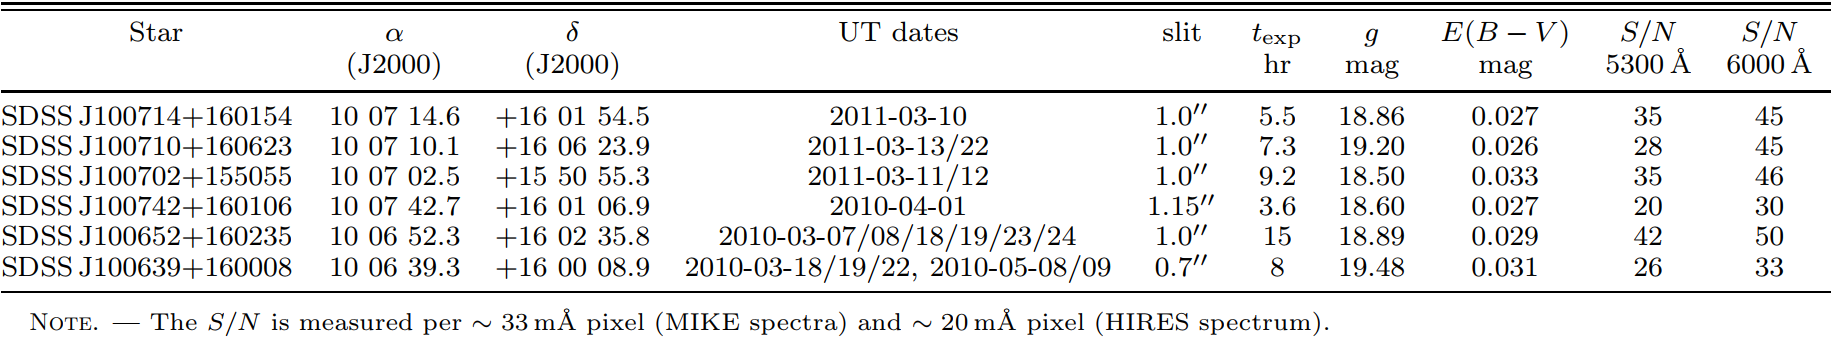
\includegraphics[width=\textwidth]{obs_detail.png}
    \caption{Observing details for the six measured stars}
    \label{table:obs_detail}
\end{table}

\section{Results and Discussion} \label{sec:dicussion}

With the high resolution spectrograph data the authors were able to extrapolate the abundances of the various elements inside the stars.
In figure 1 the authors plotted the spectra of the 6 stars compared to two other known stars, the ultra low metal $CD -38^{\circ}245$
and the very bright, and much younger, Arcturus. The plots are listed in ascending order of metallicity from top to bottom.

\begin{figure}[!h]
    \centering
    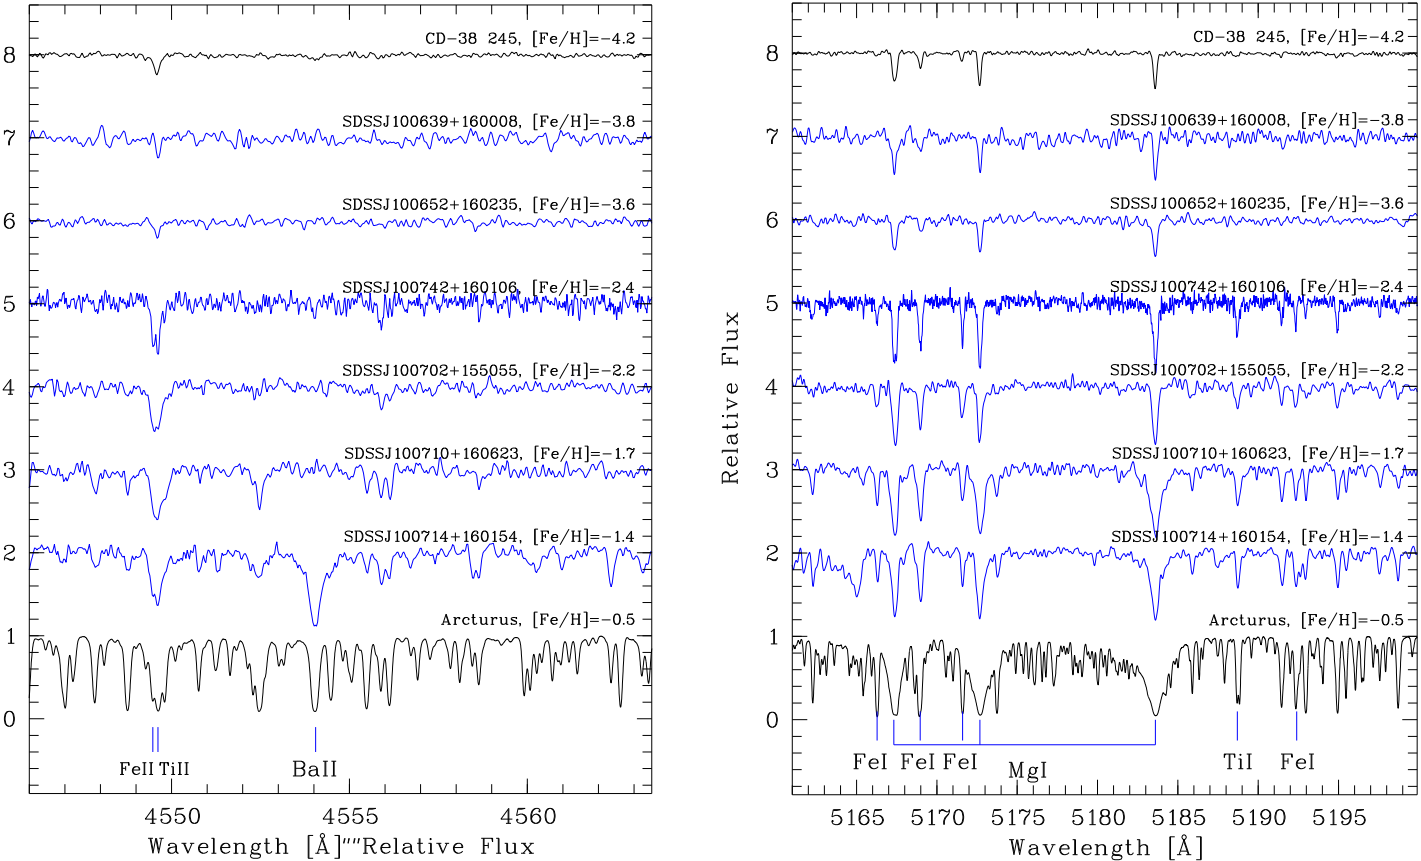
\includegraphics[width=0.85\textwidth]{spectra.png}
    \caption{Spectra of the six stars, in blue, bracketed by $CD -38^{\circ}245$ at the top and Arcturus at the bottom.
    the spectral lines of the elements are labeled at the bottom with the corresponding ranges of wavelengths.}
    \label{fig:spectra}
\end{figure}

In the three lowest metallicity stars (The top 3 blue lines) the abundance of iron (both Fe I and Fe II) is mostly indistinguishable
from the noise in the measurements. In the 3 stars with observable amounts of iron there was no correlation between increasing
iron abundance and increasing metallicity, indicated by the appearance of more spectral lines as the metallicity increases.
This indicated that there was at most one or maybe two Type Ia supernova that enriched SEGUE-1's birth cloud. This
contrasts the trend found in younger galaxies where there would be a clear trend in increasing metallicity and increasing
iron abundance in the stellar population as they evolve alongside energetic supernovae events.

Using the spectrography data the authors also plotted abundance ratios [X/Fe] relative to the iron abundance [Fe/H] for the elements
that were measured. The dashed line at [X/Fe] = 0 indicates the ratio of the element in our Sun with positive values meaning higher
abundance and lower values indicating lower abundance, on a log scale. Notice that in all of the SEGUE-1 stars the abundance of
$\alpha$-elements such as Mg, Si, Ca, and Ti, are all above that of the Sun. Elements that are synthesized by other processes that
occur later in the timeline such as Al, Cr, and Mn, have consistent abundances lower than that of the Sun.

\begin{figure}[!h]
    \centering
    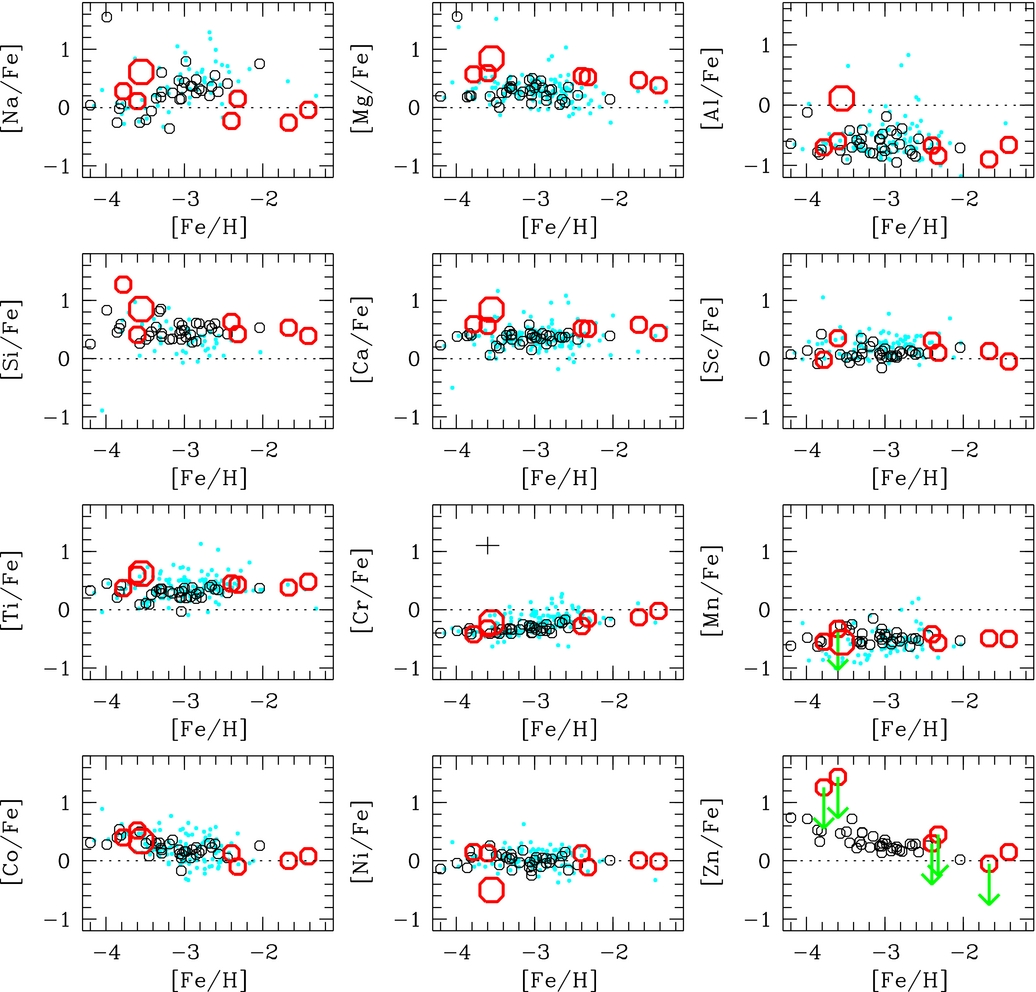
\includegraphics[width=0.6\textwidth]{elements.jpg}
    \caption{The abundance ratios [X/Fe] compared to the metallicity [Fe/H] of each of the elements that were measured with
    the spectroscopes. The six small red circles represent the SEGUE-1 stars measured in this article. The larger red circle
    is a SEGUE-1 star measured in a previous paper. The small black and blue circles represent MW halo stars measured from
    previous papers.}
    \label{fig:elements}
\end{figure}
\begin{figure}[!ht]
    \centering
    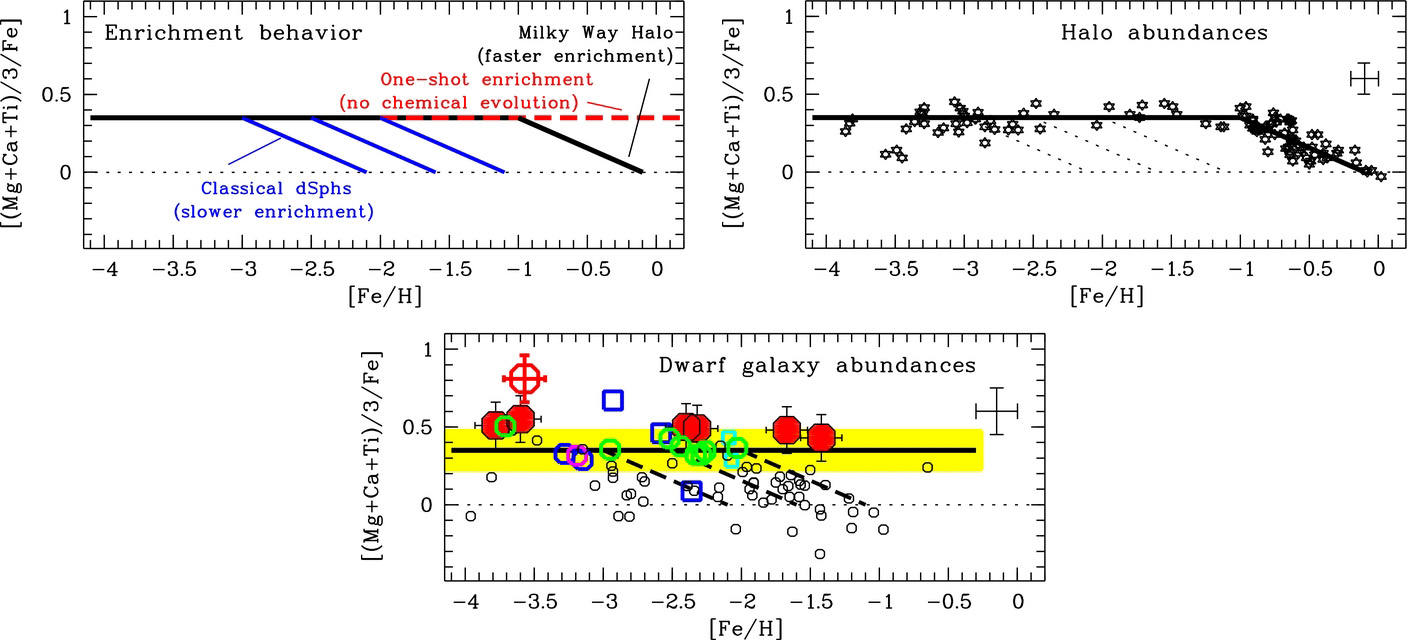
\includegraphics[width=0.8\textwidth]{enrich.jpg}
    \caption{Enrichment Behavior plots for MW Halo stars, the six measured SEGUE-1 stars, a previously measured SEGUE-1 star,
    and stars from other classical dSph galaxies. These plots show the relationship between $\alpha$-element abundance (specifically
    Mg, Ca \& Ti) ratios [$\alpha$/Fe] and the metallicity [Fe/H] within the stars.}
    \label{fig:enrich}
\end{figure}

Another indication of SEGUE-1's age is the enhanced [$\alpha$/Fe] values found in all the measured stars that are consistent with each other
and the initial birth cloud. Figure 3 shows enrichment behavior plots, [Fe/H] vs. [$\alpha$/Fe], for MW Halo stars, classical dSph galaxy stars, and SEGUE-1 stars.
The top plot in fig. 3 shows the general trend of how classical dSph galaxies and MW Halo stars will appear on the enrichment behavior plot.
The middle plot shows the spread of MW Halo stars which have a plateau in the [$\alpha$/Fe] until [Fe/H] $\approx -1$ at which point
the [$\alpha$/Fe] approaches 0 where [Fe/H] is almost at 0. The bottom plot of fig. 3 shows the enrichment behavior plot for dSph galaxy
stars (small black circles), the measured stars from SEGUE-1 (large red filled in circles from this article, and red crosshair from
previous papers), and some other candidate stars (blue square, green circles, and magenta circles). In this bottom plot we can see that
the classical dSph stars and some of the other candidate stars have a plateau but do slope down towards the [$\alpha$/Fe] = 0 line.
On the other hand, the 6 measured stars from SEGUE-1 all reside around the [$\alpha$/Fe] = 0.5 line, even past the point where MW
Halo starts to slope down on the [Fe/H] axis. The consistent [$\alpha$/Fe] values in SEGUE-1 stars suggest that after the initial
enrichment of the birth cloud there were no other enrichment events, such as type Ia supernovae, in SEGUE-1.

\begin{wrapfigure}{r}{0.4\textwidth}
    \begin{center}
        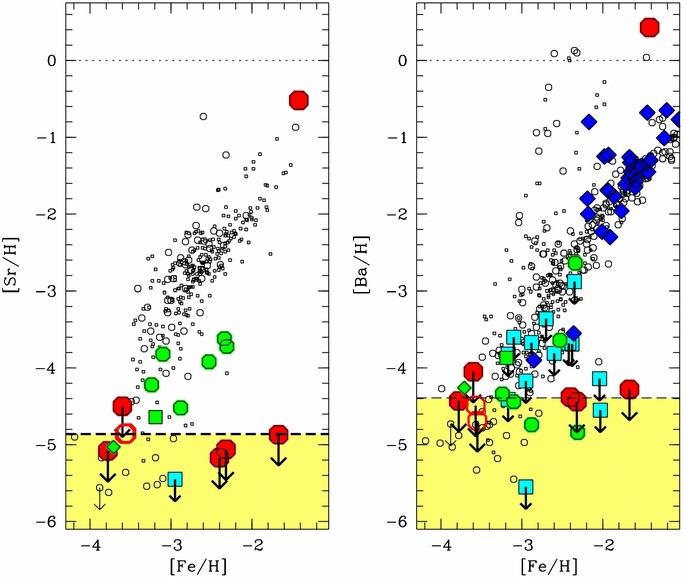
\includegraphics[width=0.38\textwidth]{neutron_cap.jpg}
    \end{center}
    \caption{Birds}
    \label{fig:neutron_cap}
\end{wrapfigure}

The final indicator of SEGUE-1's old age is the low abundance of neutron-capture elements in SEGUE's non-binary system stars,
which total to less than \(\sim 10^{-7} M_{\odot}\) for each element, indicate that there were no neutron-capture element producing
process, which produce \(\sim 10^{-4} M_{\odot}\) of neutron-capture elements per event, that occurred during the star formation phase.

\section{Future Work} \label{sec:future}

Future research points to observing a larger portion of SEGUE 1 stars. The six stars that were observed in this paper were deemed to
be the brightest in the ultra faint dwarf galaxy and only allowed for a moderate S/N values between 20 and 46. In order to observe the other, dimmer,
stars in SEGUE 1 we would require better telescopes to overcome the noise.

%% For this sample we use BibTeX plus aasjournals.bst to generate the
%% the bibliography. The sample63.bib file was populated from ADS. To
%% get the citations to show in the compiled file do the following:
%%
%% pdflatex sample63.tex
%% bibtext sample63
%% pdflatex sample63.tex
%% pdflatex sample63.tex

\nocite{*}
\bibliography{bibliography}{}
\bibliographystyle{aasjournal}

%% This command is needed to show the entire author+affiliation list when
%% the collaboration and author truncation commands are used.  It has to
%% go at the end of the manuscript.
%\allauthors

%% Include this line if you are using the \added, \replaced, \deleted
%% commands to see a summary list of all changes at the end of the article.
%\listofchanges

\end{document}